\documentclass{beamer}
\usepackage{ctex, hyperref}
\usepackage[T1]{fontenc}

% other packages
\usepackage{latexsym,amsmath,xcolor,multicol,booktabs,calligra}
\usepackage{graphicx,pstricks,listings,stackengine,newtxtext,newtxmath}

\author{赵万春}
\title{会计中的创新}
\subtitle{}
\institute{天津财经大学 金融学院}
\date{2024年5月24日}
\usepackage{tufe}

% defs
\def\cmd#1{\texttt{\color{red}\footnotesize $\backslash$#1}}
\def\env#1{\texttt{\color{blue}\footnotesize #1}}
\definecolor{deepblue}{rgb}{0,0,0.5}
\definecolor{deepred}{rgb}{0.6,0,0}
\definecolor{deepgreen}{rgb}{0,0.5,0}
\definecolor{halfgray}{gray}{0.55}

\lstset{
	basicstyle=\ttfamily\small,
	keywordstyle=\bfseries\color{deepblue},
	emphstyle=\ttfamily\color{deepred},    % Custom highlighting style
	stringstyle=\color{deepgreen},
	numbers=left,
	numberstyle=\small\color{halfgray},
	rulesepcolor=\color{red!20!green!20!blue!20},
	frame=shadowbox,
}
\usefonttheme[onlymath]{serif}

\begin{document}
	
\kaishu

\begin{frame}
	\titlepage
	\begin{figure}[htpb]
		\begin{center}
			
\includegraphics[width=0.2\linewidth]{pic/TJUFE_logo.png}
		\end{center}
	\end{figure}
\end{frame}	
	
\section{introduction}

\begin{frame}{文献概况}
	本文综述了创新研究的会计文献。
	\begin{center}
		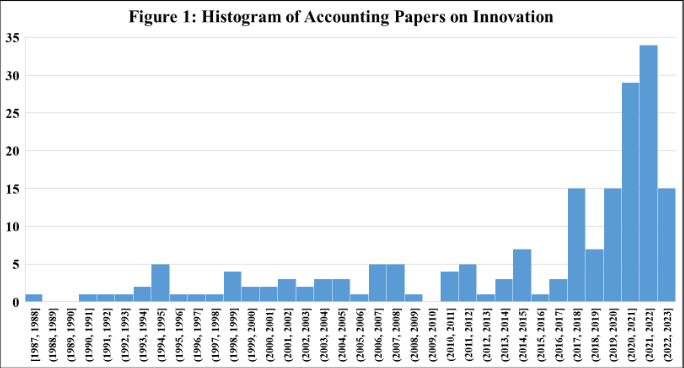
\includegraphics[width=0.6\linewidth]{pic/fig1.png}
	\end{center}
	\begin{flushleft}
		然而尽管文献数量增长迅速,但少有文献关注创新资产与其他资产的区别,以及会计人员的独特技能如何为更广泛的创新文献做出贡献。
	\end{flushleft}
\end{frame}

\begin{frame}{研究对象}
	本文专注于创新与其他资产不同的经济特征:\\
	\begin{itemize}
		\item 新颖性:新的想法或实现现有想法的新方法.
		\item 非竞争性:多方同时使用一项创新成果,却不损害各方获取创新成果的能力(Samulson,1954)
		\item 部分排他性。创新所有者无法完全合法地限制他人获取其创新(产权)
	\end{itemize}
	创新的经济学特征导致了许多经济学上的挑战。
\end{frame}

\begin{frame}{创新与宏观经济学}
	传统宏观经济学中,生产使用劳动和资本两种对立要素。\\
	如果没有创新,增长就会受到可用劳动力和资本存量增长的限制。\\
	因此,随着人口增长,人均产出保持不变,甚至由于边际收益递减而下降。\\
	然而人均资本产出并没有下降(Bolt et al.,2020)\\
	\begin{center}
		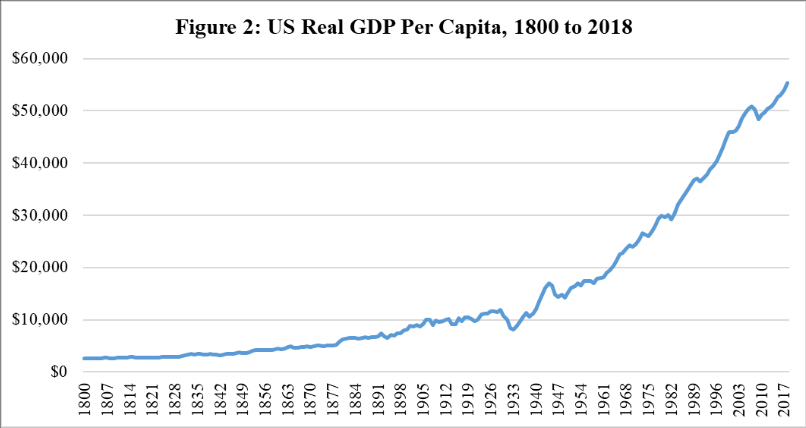
\includegraphics[width=0.6\linewidth]{pic/fig2.png}
	\end{center}
\end{frame}

\begin{frame}{用创新解释增长}
	首先,创新可以在不损害可用性的情况下被复用。\\
	进一步,新的创新可以利用之前的创新,实现创新之间的互动,促进增长(Jones,2023)\\
	最后,创新存在知识溢出效应,有利于驱动经济增长。\\
	最近的一个例子是,人工智能(AI)的非竞争性促进了人工智能在现代经济中的传播;截至 2023 年 6 月 1 日,美国市值最大的五家公司分别是苹果、微软、Alphabet、亚马逊和英伟达,它们都利用了人工智能和其他创新的各个方面。
\end{frame}

\begin{frame}{为什么创新对于会计研究很重要?}
	\alert{创新的新颖性、非竞争性和部分排他性导致了会计信息问题。}
	\begin{itemize}
		\item 部分排他和非竞争性导致了知识溢出(Romer,1990)。
		\item 进一步,创新披露会通过知识溢出产生正外部性(Dyer et al., 2020; Kim and Valentine, 2021)
		\item 创新披露为创新主体带来产权成本
		\item 部分排他性允许他人侵占创新的部分价值,事前阻碍了创新。
	\end{itemize}
	产权成本和创新披露收益权衡是会计研究的重要议题之一(Verrechia,1983)
\end{frame}

\begin{frame}{创新与制度}
	创新的新颖性导致企业不能完全控制创新收益。\\
	创新的产权成本和披露的正外部性,导致创新的法律与税收机制设计具有复杂性。\\
	创新的新颖性导致事前签订的契约必然不完善(Aghion and Tirole, 1994),为会计研究带来了挑战(Christensen et al., 2016)\\
	\alert{许多看似关系不大的难题都源于创新的新颖性。}
\end{frame}

\begin{frame}{测度创新}
	\begin{itemize}
		\item 创新的部分排他性阻碍了公开披露,
		\item 创新的新颖性使经验比较变得复杂,
		\item 创新的非竞争性意味着许多创新并不明确属于哪家公司,也不在哪家公司的范围内运作。
	\end{itemize}
	衡量创新的最佳方法因研究问题和研究环境的不同而不同。\\
	开发新的实证技术、数据集和可信外生变量来源的研究机会。
\end{frame}

\begin{frame}{新的研究视角}
	披露、搜索和契约:信息与创新(Romer,1990;Jones,2023)\\
	\begin{itemize}
		\item 非正式公开:盗用与逆向工程
		\item 基于会计信息的契约理论与增长理论创新
	\end{itemize}
	AI如何影响信息过程与创新(Blankespoor et al., 2020)
	\begin{itemize}
		\item[] AI改变了财报、契约与审计(Fedyk et al., 2022)
		\item[] AI也可能通过识别创新机会,直接影响创新与增长
	\end{itemize}
	企业如何与个人发明者订立契约?
	\begin{itemize}
		\item 部分排他导致的成果挪用
		\item 激励机制与契约设计问题,控制问题。
	\end{itemize}
\end{frame}

\begin{frame}{既有视角的新拓展}
	关注创新的部分排他性和非竞争性的研究较少。\\
	为什么某些公司不利用创新的非竞争性和新颖性避税?\\
	鼓励创新和披露创新的税收和非税收政策最优组合是什么?\\
	ESG与创新(Christensen et al., 2021)
\end{frame}

\section{What is Innovation?}

\subsection{Defining Innovation}

\begin{frame}{定义创新}
	创新:\alert{改进生产流程、产品、方法或平台的新想法。}(Arrow,1962; Romer,1990)\\
	创新具有\alert{新颖性、非竞争性和部分排他性}。(Romer, 1990; Aghion and Tirole, 1994)
	\begin{itemize}
		\item 新颖性:创新必须是特定背景下企业、实体或社会的新事物。
		\item 非竞争性:一方使用不影响他人创新的数量、质量或可用性。
		\item 部分排他性:创新所有者无法完全限制他人合法使用其创新。
	\end{itemize}
\end{frame}

\begin{frame}{什么是创新,什么不是创新?}
	依托创新的有形产品和机器都不是创新(具有竞争性、排他性)
	\begin{itemize}
		\item[] T型车和生产T型车的产线都不是创新。
		\item[] 生产T型车的idea属于创新。
	\end{itemize}
	创新是一种知识产权和无形资产,但反推不一定。
	\begin{itemize}
		\item[] 客户名单、数据库、商标、广告和常识都具有创新特征,但不是创新。
		\item[] 要么不是idea(客户名单和数据库)
		\item[] 要么不具有新颖性(客户名单是已知数据的集合)
	\end{itemize}
	“技术”(Romer, 1990; Jones, 2023)不能用于指代创新,因为技术具有竞争性。
\end{frame}

\subsection{Measurement}

\begin{frame}{测度创新:概述}
	对创新测度的三种批评
	\begin{itemize}
		\item 部分指标只反映了创新的排他性(专利与商业秘密权),而非部分排他性。
		\item 大部分研究强调上市公司的创新
		\item 数据质量和排他性存在正相关
	\end{itemize}
	创新生命周期
	\begin{center}
		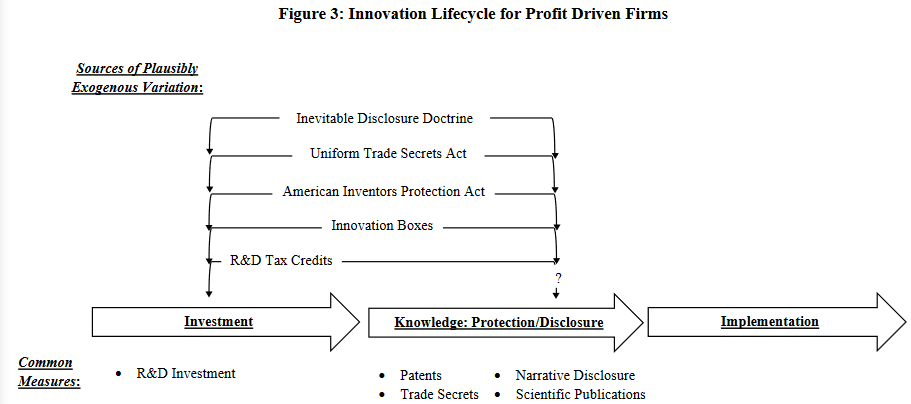
\includegraphics[width=0.8\linewidth]{pic/fig3.png}
	\end{center}
\end{frame}

\begin{frame}{创新投资:R\&D支出与存量}
	最典型的测度是研发费用。
	\begin{itemize}
		\item[] 数据广泛、通用性强
		\item[] 披露相对粗糙,无法观测创新方向、创新披露与其他问题。
		\item[] 不能反映创新是否成功
	\end{itemize}
	研发费用是一个流量变量,但使用R\&D存量有时更精确。
	\begin{itemize}
		\item 累计研发费用+折旧,估算研发存量
		\item[] 选择直接折旧或者行业折旧(Li and Hall,2020)
		\item[] 独立估算折旧率的文章较少(Ewens et al. ,2019; Iqbal et al. ,2023)
	\end{itemize}
\end{frame}

\begin{frame}{研发费用与折旧的适用场景}
	话题1:研发费用资本化与折旧
	\begin{itemize}
		\item 研发折旧与创新类型的相关性
		\item 不同市场势力企业的研发策略差异
		\item 征用可能性(expropriation likelihoods)
		\item 研发费用资本化背景下的折旧率策略性选择
	\end{itemize}
	话题2:研发费用与政策
	\begin{itemize}
		\item 研发费用折旧与私人知识汇报下降
		\item 在新的无形资产定义背景下,研发资本折旧对允许研发费用资本化的影响。
	\end{itemize}
\end{frame}

\begin{frame}{研发费用与折旧的劣势}
\begin{list}{label}{spacing}
	\item 	许多企业不在财报中列示研发费用
	不重要还是没有?(Koh and Reeb, 2015)\\
\end{list}
	
\end{frame}
\begin{frame}{文献概述}
	Ewens et al.(2019)利用并购中的市场价格和并购价格分配以及破产恢复数据,估算无形资产价值和行业折旧率
	Iqbal et al.(2023)利用行业—年度回归分析了无形投资与未来收入之间的关系。
\end{frame}
\end{document}